\documentclass[tikz,border=2pt]{standalone}
\usepackage{amsmath,amssymb}
\usepackage{pgfplots}
\pgfplotsset{compat=1.18}
\usetikzlibrary{arrows.meta}
\begin{document}
% Jar of coins: v=100, theta_i = 100+eps_i with eps_i iid U[-20,20], n=3. One estimate is
% uniform on [80,120] with mean 100; the largest of three has density 3(x-80)^2/40^3 on [80,120]
% with mean 110, so a winner who bids her estimate pays 10 too much on average.
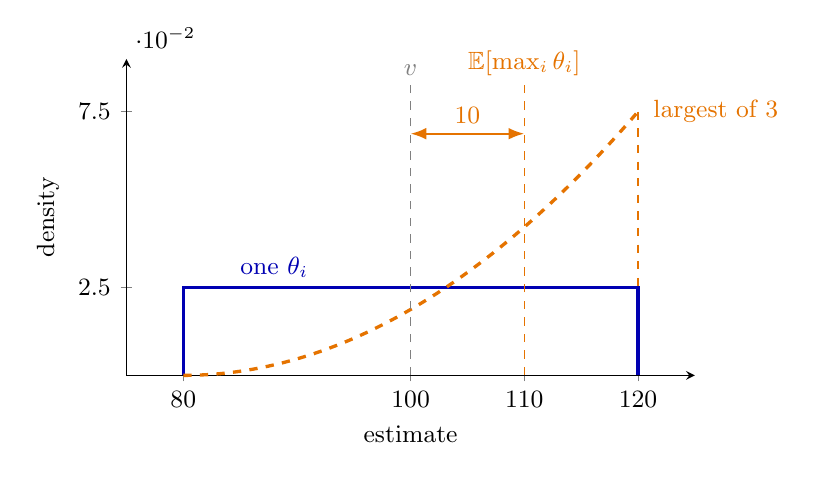
\begin{tikzpicture}[font=\small, >={Latex[length=2mm]}]
  \begin{axis}[width=8.8cm, height=5.6cm, axis lines=left,
      xmin=75, xmax=125, ymin=0, ymax=0.09,
      xtick={80,100,110,120}, ytick={0.025,0.075},
      xlabel={estimate}, ylabel={density},
      clip=false]
    % one estimate theta_i
    \draw[very thick, blue!70!black] (axis cs:80,0) -- (axis cs:80,0.025) -- (axis cs:120,0.025) -- (axis cs:120,0);
    % largest of the three estimates
    \addplot[very thick, orange!90!black, dashed, domain=80:120, samples=60] {3*((x-80)/40)^2/40};
    \draw[orange!90!black, thin, dashed] (axis cs:120,0.075) -- (axis cs:120,0.025);
    % means
    \draw[gray, dashed] (axis cs:100,0) -- (axis cs:100,0.0825);
    \draw[orange!90!black, dashed] (axis cs:110,0) -- (axis cs:110,0.0825);
    \draw[<->, thick, orange!90!black] (axis cs:100,0.06875) -- (axis cs:110,0.06875)
      node[midway, above] {$10$};
    \node[gray, anchor=south] at (axis cs:100,0.0825) {$v$};
    \node[orange!90!black, anchor=south] at (axis cs:110,0.0825) {$\mathbb{E}[\max_i\theta_i]$};
    \node[blue!70!black, anchor=south] at (axis cs:88,0.025) {one $\theta_i$};
    \node[orange!90!black, anchor=west] at (axis cs:120.5,0.075) {largest of $3$};
  \end{axis}
\end{tikzpicture}
\end{document}
